% Created by tikzDevice version 0.12.3 on 2020-04-10 11:40:59
% !TEX encoding = UTF-8 Unicode
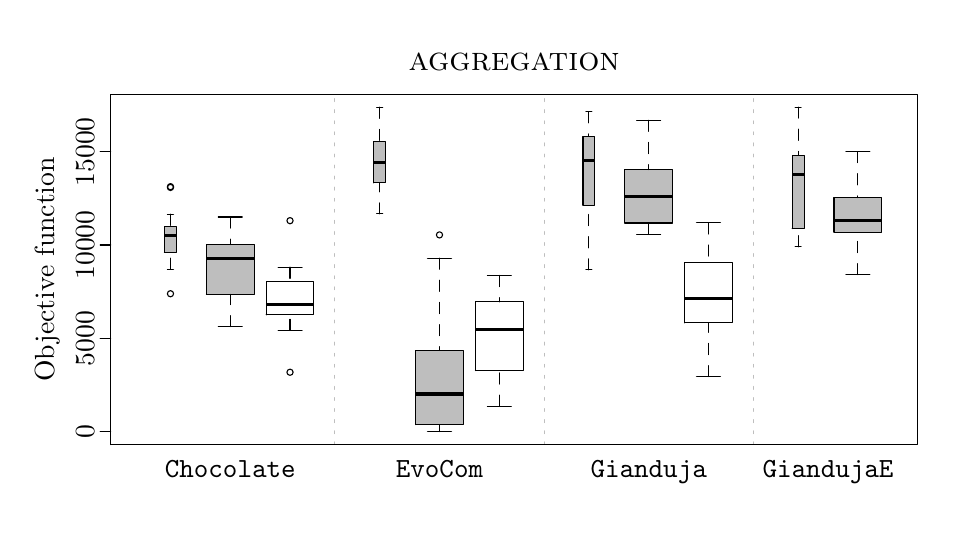
\begin{tikzpicture}[x=1pt,y=1pt]
\definecolor{fillColor}{RGB}{255,255,255}
\path[use as bounding box,fill=fillColor,fill opacity=0.00] (0,0) rectangle (325.21,180.67);
\begin{scope}
\path[clip] ( 30.00, 30.00) rectangle (321.61,156.67);
\definecolor{fillColor}{RGB}{190,190,190}

\path[fill=fillColor] ( 49.44, 99.54) --
	( 53.76, 99.54) --
	( 53.76,108.76) --
	( 49.44,108.76) --
	cycle;
\definecolor{drawColor}{RGB}{0,0,0}

\path[draw=drawColor,line width= 1.2pt,line join=round] ( 49.44,105.45) -- ( 53.76,105.45);

\path[draw=drawColor,line width= 0.4pt,dash pattern=on 4pt off 4pt ,line join=round,line cap=round] ( 51.60, 93.37) -- ( 51.60, 99.54);

\path[draw=drawColor,line width= 0.4pt,dash pattern=on 4pt off 4pt ,line join=round,line cap=round] ( 51.60,113.25) -- ( 51.60,108.76);

\path[draw=drawColor,line width= 0.4pt,line join=round,line cap=round] ( 50.52, 93.37) -- ( 52.68, 93.37);

\path[draw=drawColor,line width= 0.4pt,line join=round,line cap=round] ( 50.52,113.25) -- ( 52.68,113.25);

\path[draw=drawColor,line width= 0.4pt,line join=round,line cap=round] ( 49.44, 99.54) --
	( 53.76, 99.54) --
	( 53.76,108.76) --
	( 49.44,108.76) --
	( 49.44, 99.54);

\path[draw=drawColor,line width= 0.4pt,line join=round,line cap=round] ( 51.60, 84.53) circle (  1.12);

\path[draw=drawColor,line width= 0.4pt,line join=round,line cap=round] ( 51.60,123.22) circle (  1.12);

\path[draw=drawColor,line width= 0.4pt,line join=round,line cap=round] ( 51.60,122.94) circle (  1.12);

\path[fill=fillColor] ( 64.56, 84.30) --
	( 81.84, 84.30) --
	( 81.84,102.25) --
	( 64.56,102.25) --
	cycle;

\path[draw=drawColor,line width= 1.2pt,line join=round] ( 64.56, 97.16) -- ( 81.84, 97.16);

\path[draw=drawColor,line width= 0.4pt,dash pattern=on 4pt off 4pt ,line join=round,line cap=round] ( 73.20, 72.63) -- ( 73.20, 84.30);

\path[draw=drawColor,line width= 0.4pt,dash pattern=on 4pt off 4pt ,line join=round,line cap=round] ( 73.20,112.24) -- ( 73.20,102.25);

\path[draw=drawColor,line width= 0.4pt,line join=round,line cap=round] ( 68.88, 72.63) -- ( 77.52, 72.63);

\path[draw=drawColor,line width= 0.4pt,line join=round,line cap=round] ( 68.88,112.24) -- ( 77.52,112.24);

\path[draw=drawColor,line width= 0.4pt,line join=round,line cap=round] ( 64.56, 84.30) --
	( 81.84, 84.30) --
	( 81.84,102.25) --
	( 64.56,102.25) --
	( 64.56, 84.30);
\definecolor{fillColor}{RGB}{255,255,255}

\path[fill=fillColor] ( 86.16, 76.88) --
	(103.44, 76.88) --
	(103.44, 88.86) --
	( 86.16, 88.86) --
	cycle;

\path[draw=drawColor,line width= 1.2pt,line join=round] ( 86.16, 80.73) -- (103.44, 80.73);

\path[draw=drawColor,line width= 0.4pt,dash pattern=on 4pt off 4pt ,line join=round,line cap=round] ( 94.80, 71.28) -- ( 94.80, 76.88);

\path[draw=drawColor,line width= 0.4pt,dash pattern=on 4pt off 4pt ,line join=round,line cap=round] ( 94.80, 94.09) -- ( 94.80, 88.86);

\path[draw=drawColor,line width= 0.4pt,line join=round,line cap=round] ( 90.48, 71.28) -- ( 99.12, 71.28);

\path[draw=drawColor,line width= 0.4pt,line join=round,line cap=round] ( 90.48, 94.09) -- ( 99.12, 94.09);

\path[draw=drawColor,line width= 0.4pt,line join=round,line cap=round] ( 86.16, 76.88) --
	(103.44, 76.88) --
	(103.44, 88.86) --
	( 86.16, 88.86) --
	( 86.16, 76.88);

\path[draw=drawColor,line width= 0.4pt,line join=round,line cap=round] ( 94.80, 56.16) circle (  1.12);

\path[draw=drawColor,line width= 0.4pt,line join=round,line cap=round] ( 94.80,110.93) circle (  1.12);
\definecolor{fillColor}{RGB}{190,190,190}

\path[fill=fillColor] (125.04,124.61) --
	(129.37,124.61) --
	(129.37,139.52) --
	(125.04,139.52) --
	cycle;

\path[draw=drawColor,line width= 1.2pt,line join=round] (125.04,132.00) -- (129.37,132.00);

\path[draw=drawColor,line width= 0.4pt,dash pattern=on 4pt off 4pt ,line join=round,line cap=round] (127.20,113.38) -- (127.20,124.61);

\path[draw=drawColor,line width= 0.4pt,dash pattern=on 4pt off 4pt ,line join=round,line cap=round] (127.20,151.91) -- (127.20,139.52);

\path[draw=drawColor,line width= 0.4pt,line join=round,line cap=round] (126.12,113.38) -- (128.29,113.38);

\path[draw=drawColor,line width= 0.4pt,line join=round,line cap=round] (126.12,151.91) -- (128.29,151.91);

\path[draw=drawColor,line width= 0.4pt,line join=round,line cap=round] (125.04,124.61) --
	(129.37,124.61) --
	(129.37,139.52) --
	(125.04,139.52) --
	(125.04,124.61);

\path[fill=fillColor] (140.17, 37.23) --
	(157.45, 37.23) --
	(157.45, 64.06) --
	(140.17, 64.06) --
	cycle;

\path[draw=drawColor,line width= 1.2pt,line join=round] (140.17, 48.35) -- (157.45, 48.35);

\path[draw=drawColor,line width= 0.4pt,dash pattern=on 4pt off 4pt ,line join=round,line cap=round] (148.81, 34.69) -- (148.81, 37.23);

\path[draw=drawColor,line width= 0.4pt,dash pattern=on 4pt off 4pt ,line join=round,line cap=round] (148.81, 97.39) -- (148.81, 64.06);

\path[draw=drawColor,line width= 0.4pt,line join=round,line cap=round] (144.49, 34.69) -- (153.13, 34.69);

\path[draw=drawColor,line width= 0.4pt,line join=round,line cap=round] (144.49, 97.39) -- (153.13, 97.39);

\path[draw=drawColor,line width= 0.4pt,line join=round,line cap=round] (140.17, 37.23) --
	(157.45, 37.23) --
	(157.45, 64.06) --
	(140.17, 64.06) --
	(140.17, 37.23);

\path[draw=drawColor,line width= 0.4pt,line join=round,line cap=round] (148.81,105.79) circle (  1.12);
\definecolor{fillColor}{RGB}{255,255,255}

\path[fill=fillColor] (161.77, 56.73) --
	(179.05, 56.73) --
	(179.05, 81.60) --
	(161.77, 81.60) --
	cycle;

\path[draw=drawColor,line width= 1.2pt,line join=round] (161.77, 71.65) -- (179.05, 71.65);

\path[draw=drawColor,line width= 0.4pt,dash pattern=on 4pt off 4pt ,line join=round,line cap=round] (170.41, 43.91) -- (170.41, 56.73);

\path[draw=drawColor,line width= 0.4pt,dash pattern=on 4pt off 4pt ,line join=round,line cap=round] (170.41, 91.11) -- (170.41, 81.60);

\path[draw=drawColor,line width= 0.4pt,line join=round,line cap=round] (166.09, 43.91) -- (174.73, 43.91);

\path[draw=drawColor,line width= 0.4pt,line join=round,line cap=round] (166.09, 91.11) -- (174.73, 91.11);

\path[draw=drawColor,line width= 0.4pt,line join=round,line cap=round] (161.77, 56.73) --
	(179.05, 56.73) --
	(179.05, 81.60) --
	(161.77, 81.60) --
	(161.77, 56.73);
\definecolor{fillColor}{RGB}{190,190,190}

\path[fill=fillColor] (200.65,116.57) --
	(204.97,116.57) --
	(204.97,141.42) --
	(200.65,141.42) --
	cycle;

\path[draw=drawColor,line width= 1.2pt,line join=round] (200.65,132.60) -- (204.97,132.60);

\path[draw=drawColor,line width= 0.4pt,dash pattern=on 4pt off 4pt ,line join=round,line cap=round] (202.81, 93.15) -- (202.81,116.57);

\path[draw=drawColor,line width= 0.4pt,dash pattern=on 4pt off 4pt ,line join=round,line cap=round] (202.81,150.31) -- (202.81,141.42);

\path[draw=drawColor,line width= 0.4pt,line join=round,line cap=round] (201.73, 93.15) -- (203.89, 93.15);

\path[draw=drawColor,line width= 0.4pt,line join=round,line cap=round] (201.73,150.31) -- (203.89,150.31);

\path[draw=drawColor,line width= 0.4pt,line join=round,line cap=round] (200.65,116.57) --
	(204.97,116.57) --
	(204.97,141.42) --
	(200.65,141.42) --
	(200.65,116.57);

\path[fill=fillColor] (215.77,110.08) --
	(233.05,110.08) --
	(233.05,129.38) --
	(215.77,129.38) --
	cycle;

\path[draw=drawColor,line width= 1.2pt,line join=round] (215.77,119.54) -- (233.05,119.54);

\path[draw=drawColor,line width= 0.4pt,dash pattern=on 4pt off 4pt ,line join=round,line cap=round] (224.41,106.06) -- (224.41,110.08);

\path[draw=drawColor,line width= 0.4pt,dash pattern=on 4pt off 4pt ,line join=round,line cap=round] (224.41,147.20) -- (224.41,129.38);

\path[draw=drawColor,line width= 0.4pt,line join=round,line cap=round] (220.09,106.06) -- (228.73,106.06);

\path[draw=drawColor,line width= 0.4pt,line join=round,line cap=round] (220.09,147.20) -- (228.73,147.20);

\path[draw=drawColor,line width= 0.4pt,line join=round,line cap=round] (215.77,110.08) --
	(233.05,110.08) --
	(233.05,129.38) --
	(215.77,129.38) --
	(215.77,110.08);
\definecolor{fillColor}{RGB}{255,255,255}

\path[fill=fillColor] (237.37, 74.03) --
	(254.65, 74.03) --
	(254.65, 95.88) --
	(237.37, 95.88) --
	cycle;

\path[draw=drawColor,line width= 1.2pt,line join=round] (237.37, 82.80) -- (254.65, 82.80);

\path[draw=drawColor,line width= 0.4pt,dash pattern=on 4pt off 4pt ,line join=round,line cap=round] (246.01, 54.56) -- (246.01, 74.03);

\path[draw=drawColor,line width= 0.4pt,dash pattern=on 4pt off 4pt ,line join=round,line cap=round] (246.01,110.12) -- (246.01, 95.88);

\path[draw=drawColor,line width= 0.4pt,line join=round,line cap=round] (241.69, 54.56) -- (250.33, 54.56);

\path[draw=drawColor,line width= 0.4pt,line join=round,line cap=round] (241.69,110.12) -- (250.33,110.12);

\path[draw=drawColor,line width= 0.4pt,line join=round,line cap=round] (237.37, 74.03) --
	(254.65, 74.03) --
	(254.65, 95.88) --
	(237.37, 95.88) --
	(237.37, 74.03);
\definecolor{fillColor}{RGB}{190,190,190}

\path[fill=fillColor] (276.25,108.03) --
	(280.57,108.03) --
	(280.57,134.53) --
	(276.25,134.53) --
	cycle;

\path[draw=drawColor,line width= 1.2pt,line join=round] (276.25,127.50) -- (280.57,127.50);

\path[draw=drawColor,line width= 0.4pt,dash pattern=on 4pt off 4pt ,line join=round,line cap=round] (278.41,101.51) -- (278.41,108.03);

\path[draw=drawColor,line width= 0.4pt,dash pattern=on 4pt off 4pt ,line join=round,line cap=round] (278.41,151.98) -- (278.41,134.53);

\path[draw=drawColor,line width= 0.4pt,line join=round,line cap=round] (277.33,101.51) -- (279.49,101.51);

\path[draw=drawColor,line width= 0.4pt,line join=round,line cap=round] (277.33,151.98) -- (279.49,151.98);

\path[draw=drawColor,line width= 0.4pt,line join=round,line cap=round] (276.25,108.03) --
	(280.57,108.03) --
	(280.57,134.53) --
	(276.25,134.53) --
	(276.25,108.03);

\path[fill=fillColor] (291.37,106.81) --
	(308.65,106.81) --
	(308.65,119.24) --
	(291.37,119.24) --
	cycle;

\path[draw=drawColor,line width= 1.2pt,line join=round] (291.37,110.88) -- (308.65,110.88);

\path[draw=drawColor,line width= 0.4pt,dash pattern=on 4pt off 4pt ,line join=round,line cap=round] (300.01, 91.41) -- (300.01,106.81);

\path[draw=drawColor,line width= 0.4pt,dash pattern=on 4pt off 4pt ,line join=round,line cap=round] (300.01,135.89) -- (300.01,119.24);

\path[draw=drawColor,line width= 0.4pt,line join=round,line cap=round] (295.69, 91.41) -- (304.33, 91.41);

\path[draw=drawColor,line width= 0.4pt,line join=round,line cap=round] (295.69,135.89) -- (304.33,135.89);

\path[draw=drawColor,line width= 0.4pt,line join=round,line cap=round] (291.37,106.81) --
	(308.65,106.81) --
	(308.65,119.24) --
	(291.37,119.24) --
	(291.37,106.81);
\definecolor{drawColor}{RGB}{190,190,190}

\path[draw=drawColor,line width= 0.4pt,dash pattern=on 1pt off 3pt ,line join=round,line cap=round] (111.00, 30.00) -- (111.00,156.67);

\path[draw=drawColor,line width= 0.4pt,dash pattern=on 1pt off 3pt ,line join=round,line cap=round] (186.61, 30.00) -- (186.61,156.67);

\path[draw=drawColor,line width= 0.4pt,dash pattern=on 1pt off 3pt ,line join=round,line cap=round] (262.21, 30.00) -- (262.21,156.67);
\end{scope}
\begin{scope}
\path[clip] (  0.00,  0.00) rectangle (325.21,180.67);
\definecolor{drawColor}{RGB}{0,0,0}

\node[text=drawColor,anchor=base,inner sep=0pt, outer sep=0pt, scale=  1.00] at ( 73.20, 18.00) {\texttt{Chocolate}};

\node[text=drawColor,anchor=base,inner sep=0pt, outer sep=0pt, scale=  1.00] at (148.81, 18.00) {\texttt{EvoCom}};

\node[text=drawColor,anchor=base,inner sep=0pt, outer sep=0pt, scale=  1.00] at (224.41, 18.00) {\texttt{Gianduja}};

\node[text=drawColor,anchor=base,inner sep=0pt, outer sep=0pt, scale=  1.00] at (289.21, 18.00) {\texttt{GiandujaE}};
\end{scope}
\begin{scope}
\path[clip] (  0.00,  0.00) rectangle (325.21,180.67);
\definecolor{drawColor}{RGB}{0,0,0}

\node[text=drawColor,anchor=base,inner sep=0pt, outer sep=0pt, scale=  1.20] at (175.81,165.07) {\textsc{aggregation}};

\node[text=drawColor,rotate= 90.00,anchor=base,inner sep=0pt, outer sep=0pt, scale=  1.00] at (  9.60, 93.34) {Objective function};
\end{scope}
\begin{scope}
\path[clip] (  0.00,  0.00) rectangle (325.21,180.67);
\definecolor{drawColor}{RGB}{0,0,0}

\path[draw=drawColor,line width= 0.4pt,line join=round,line cap=round] ( 30.00, 34.69) -- ( 30.00,135.83);

\path[draw=drawColor,line width= 0.4pt,line join=round,line cap=round] ( 30.00, 34.69) -- ( 26.20, 34.69);

\path[draw=drawColor,line width= 0.4pt,line join=round,line cap=round] ( 30.00, 68.41) -- ( 26.20, 68.41);

\path[draw=drawColor,line width= 0.4pt,line join=round,line cap=round] ( 30.00,102.12) -- ( 26.20,102.12);

\path[draw=drawColor,line width= 0.4pt,line join=round,line cap=round] ( 30.00,135.83) -- ( 26.20,135.83);

\node[text=drawColor,rotate= 90.00,anchor=base,inner sep=0pt, outer sep=0pt, scale=  1.00] at ( 24.00, 34.69) {0};

\node[text=drawColor,rotate= 90.00,anchor=base,inner sep=0pt, outer sep=0pt, scale=  1.00] at ( 24.00, 68.41) {5000};

\node[text=drawColor,rotate= 90.00,anchor=base,inner sep=0pt, outer sep=0pt, scale=  1.00] at ( 24.00,102.12) {10000};

\node[text=drawColor,rotate= 90.00,anchor=base,inner sep=0pt, outer sep=0pt, scale=  1.00] at ( 24.00,135.83) {15000};

\path[draw=drawColor,line width= 0.4pt,line join=round,line cap=round] ( 30.00, 30.00) --
	(321.61, 30.00) --
	(321.61,156.67) --
	( 30.00,156.67) --
	( 30.00, 30.00);
\end{scope}
\end{tikzpicture}
